\documentclass[a4paper,11pt]{article}
\usepackage{multicol}
\usepackage{pdfpages}



\begin{document}
	\title{Paarka a plataform  on the Cardano Block-Chain  for  Video and Audio Tokens }



	


	\maketitle
	



	
	
\begin{abstract}
Paarka allows content creators to publish individually unique $\&$ limited edition encrypted
videos and audio files, for this we mind Cardano native tokens to act as a license that will decrypt
or unlock those media files. 
Our platform allows you to grow  your community, incentivize marketing partners, share profits with customizable smart contracts, track engagement, buy sell and trade NFT’s and native tokens with several innovative adaptations for the Cardano Block-Chain.

\subsubsection*{A NEW MARKET FOR DIGITAL ASSETS EMERGES}


\end{abstract}
\begin{multicols}{2}	
	
	
	\subsection{Background}
	
	What is an NFT an why its a good option for sharing rights of music and video
	
	A little description of The Cardano Block-Chain, ... offers a far secure network with NFT available since ...
	
	Explain more about Cardano fees compared to ethereum
	
	And How it would be posibble to trade Tokens in a lower ranges of prices
	
	
	
	
	 
	\subsection{The Paarka Platform	}

	
	Paarka is a publishing tool for digital goods, including videos, music, and other digital assets. On Paarka, you can buy, sell, and trade any of these items with anyone in the world. Paarka is currently the only general marketplace for user-owned NFT based video and music digital goods. Paarka is also partners with various  decentralized marketplaces. Trading on on Paarka happens through a smart contract, meaning that no central authority ever holds custody of your items. Instead, users store items in their wallet of choice - whether that's a mobile wallet like Trust, Coinbase Wallet, or Opera or an in-browser chrome extension like MetaMask.
	

	
	\subsubsection{The Problem}
	Problem: distributorsdistributers/ content creators still need better solutions to market and monetize their creations and protect their digital goods from from piracy. Consumers need alternatives to streaming platforms in order to create personalized collections of movies and music with superior UX/UI.
	
	\subsubsection{The Solution}
	Solution: Digital files encrypted and licensed via NFT tokens to protect the files from piracy. The NFT tokens can be bought, sold and transferred securely, also  gamified to increase engagement.
	
	Paarka will allow publishers to create Smart contract affiliate links, which provide a way to engage marketing partners. Decentralized marketplaces remove middlemen and allow  trading of these digital assets.
	
\subsubsection{Paarka Token}
Paarka token is used to pay publishers when their NFTs are sold via credit card.



\end{multicols}
\subsection{ Implementation on the Cardano Blockchain
	} 

The Cardano implementation will consist of an DApp (Decentrilizided App )  where the creators will be available tu create, buy, sell , subastate and eventualy  gamble their NFT in different paarka-games.

Since at the moment there is not any available public Testnet  for running Smart Contracts. We will focus first in developing the smart contracts for, minting, selling, and subastating the NFT in the current Plutus state of development. We are sure that it is only mater of  weeks so that we can test the smart contract in a public Testnet, for the moment we will test them in the  PAB (Plutus Aplication Backend).

\subsubsection{Minting NFT Contract}


We will standardize all the NFT that we create in our plataform for this we will use Plutus Smart contract minting policies that will ensure once a NFT it's created under this policy it will exist only once.

We will use the metadata that is most commonly used to date, in the meantime that there comes one stardart to use, for starting we will use the following template:


\begin{minipage}[c]{\textwidth}
	
	    \begin{center}

	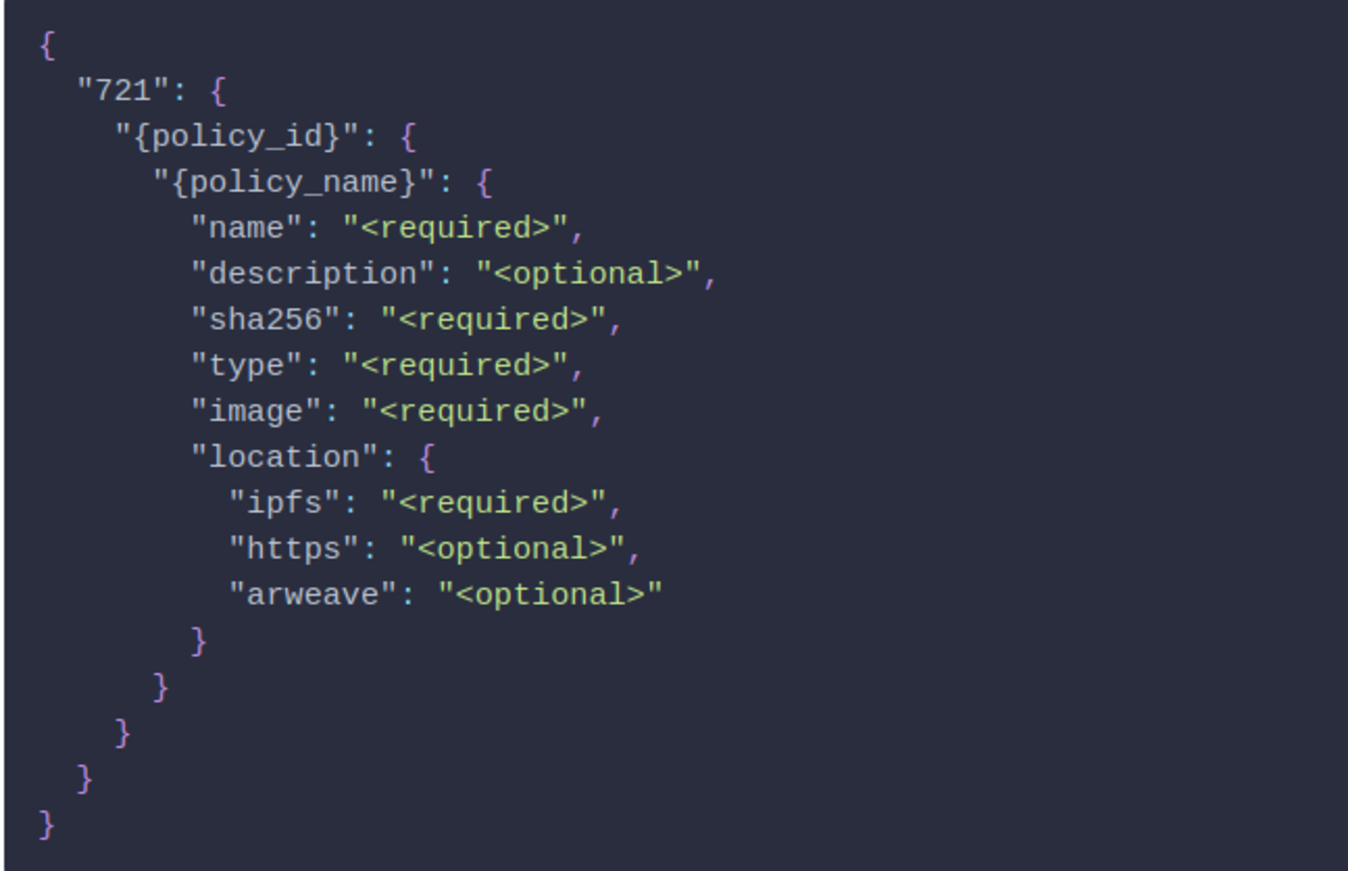
\includegraphics[scale=0.3]{metadata.pdf}


	    \end{center}
    Metadata example found in \cite{metadata}
\end{minipage}

\subsubsection{Selling NFT Contract}

This could be a state-machine contract to maintain interactions among Paarka Contract, publishers and buyers

Properties :

\begin{itemize}
\item Publisher Key of publisher
\item NFTKey: Script address of the NFT



\end{itemize}

Endpoints for the seller:

\begin{itemize}
	\item Start NFT Sale:
	\begin{itemize}
		\item to start an NFT Sale according to the parameters(properties)
		\item Interact with Paarka Contract to get the NFTToken. This should be an Asset Class, incluiding script address (Paarka Contract) and NFTKey(as token name)
	
		
	\end{itemize}
	\item setPrice: to set the price of the NFT. Only by PublisherKey
\item setDistribution: to set the distribution payment of the NFT. Only by PublisherKey.
\item retiring the NFT of sale: In case the saler decided he does not want to sell the NFT anymore
\end{itemize}
Endopoints for the buyer:

\begin{itemize}
\item buy	
\end{itemize}







\subsection{Planning for Upgrades
	}
\subsection{Future Work
	}
\subsection{Conclusion
	}
		
	

	
	

	
	\bibliographystyle{plain}
	\bibliography{mybib}
	
\end{document}
